\documentclass{article}
\usepackage{booktabs}
\usepackage{fontspec}
\begin{document}
\thispagestyle{empty}
\setromanfont{Times New Roman}
\begin{table}[htbp]
    %\ttfamily
    %
    \small
      \begin{tabular}{lrr}
        \toprule
      Methods  & Coverage & RMSD  \\
      \midrule
      DFS$_o$  & 0.65 & 3.5 \\
      DFS$_d$  & 0.68 & 3.1 \\
      DFS$_d$+PBNet  & 0.89 & 2.6 \\
      MCTS  & 0.72  & 2.9 \\
      \textbf{MCTS+PBNet}  & \textbf{0.91} & \textbf{2.0} \\

      \bottomrule
      \end{tabular}%
      %\caption{The results of detection and threading comparing with other 3D object detection methods.}
    \end{table}%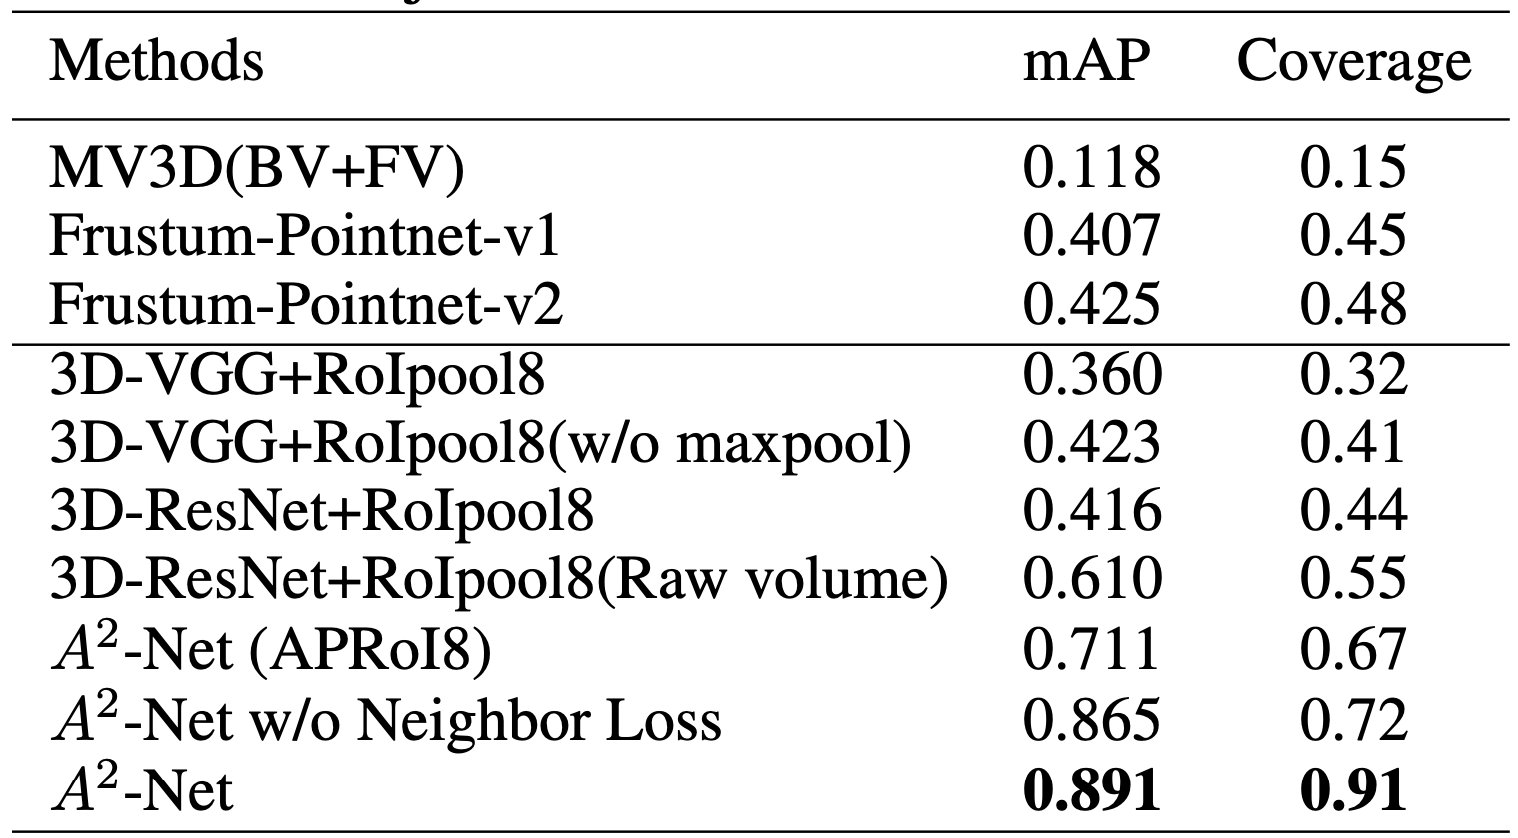
\includegraphics[width=0.45\columnwidth]{detection.png}}
\end{document}